

\tikzset{every picture/.style={line width=0.75pt}} %set default line width to 0.75pt        

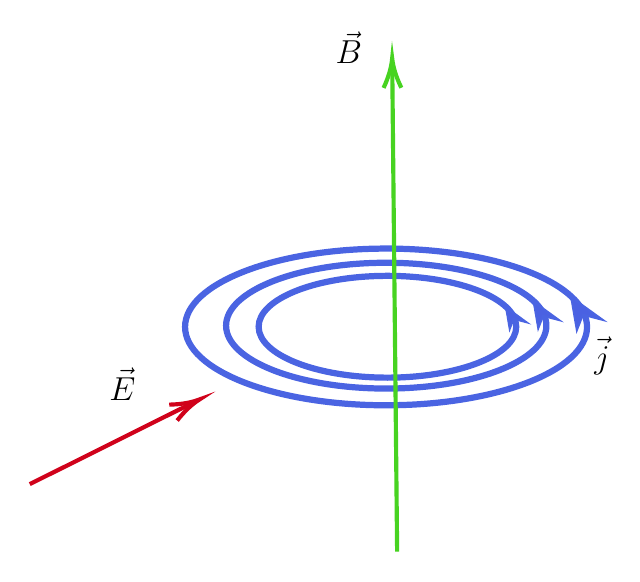
\begin{tikzpicture}[x=0.75pt,y=0.75pt,yscale=-1,xscale=1]
%uncomment if require: \path (0,300); %set diagram left start at 0, and has height of 300

%Shape: Ellipse [id:dp7618038563365439] 
\draw  [color={rgb, 255:red, 74; green, 100; blue, 226 }  ,draw opacity=1 ][line width=2.25]  (239,162.08) .. controls (239,141.23) and (282.35,124.33) .. (335.83,124.33) .. controls (389.32,124.33) and (432.67,141.23) .. (432.67,162.08) .. controls (432.67,182.93) and (389.32,199.83) .. (335.83,199.83) .. controls (282.35,199.83) and (239,182.93) .. (239,162.08) -- cycle ;
\draw  [color={rgb, 255:red, 74; green, 100; blue, 226 }  ,draw opacity=1 ][fill={rgb, 255:red, 74; green, 97; blue, 226 }  ,fill opacity=1 ] (427.77,163.58) -- (425.05,147.77) -- (440.17,158.66) -- (430.67,156.18) -- cycle ;
%Shape: Ellipse [id:dp40950593076291275] 
\draw  [color={rgb, 255:red, 74; green, 100; blue, 226 }  ,draw opacity=1 ][line width=2.25]  (258.76,161.46) .. controls (258.76,144.73) and (293.31,131.16) .. (335.92,131.16) .. controls (378.52,131.16) and (413.07,144.73) .. (413.07,161.46) .. controls (413.07,178.2) and (378.52,191.77) .. (335.92,191.77) .. controls (293.31,191.77) and (258.76,178.2) .. (258.76,161.46) -- cycle ;
\draw  [color={rgb, 255:red, 74; green, 100; blue, 226 }  ,draw opacity=1 ][fill={rgb, 255:red, 74; green, 97; blue, 226 }  ,fill opacity=1 ] (409.17,162.67) -- (406.99,149.97) -- (419.04,158.72) -- (411.47,156.73) -- cycle ;
%Shape: Ellipse [id:dp350415193172229] 
\draw  [color={rgb, 255:red, 74; green, 100; blue, 226 }  ,draw opacity=1 ][line width=2.25]  (274.44,161.99) .. controls (274.44,148.45) and (302.22,137.47) .. (336.5,137.47) .. controls (370.77,137.47) and (398.56,148.45) .. (398.56,161.99) .. controls (398.56,175.53) and (370.77,186.51) .. (336.5,186.51) .. controls (302.22,186.51) and (274.44,175.53) .. (274.44,161.99) -- cycle ;
\draw  [color={rgb, 255:red, 74; green, 100; blue, 226 }  ,draw opacity=1 ][fill={rgb, 255:red, 74; green, 97; blue, 226 }  ,fill opacity=1 ] (395.42,162.96) -- (393.67,152.69) -- (403.36,159.77) -- (397.28,158.16) -- cycle ;

%Straight Lines [id:da6004675395388991] 
\draw [color={rgb, 255:red, 71; green, 211; blue, 33 }  ,draw opacity=1 ][fill={rgb, 255:red, 68; green, 211; blue, 33 }  ,fill opacity=1 ][line width=1.5]    (341.17,270.33) -- (338.81,35.67) ;
\draw [shift={(338.78,32.67)}, rotate = 449.43] [color={rgb, 255:red, 71; green, 211; blue, 33 }  ,draw opacity=1 ][line width=1.5]    (14.21,-4.28) .. controls (9.04,-1.82) and (4.3,-0.39) .. (0,0) .. controls (4.3,0.39) and (9.04,1.82) .. (14.21,4.28)   ;
%Straight Lines [id:da8123571653101612] 
\draw [color={rgb, 255:red, 208; green, 2; blue, 27 }  ,draw opacity=1 ][line width=1.5]    (164.17,237.83) -- (243.32,198.34) ;
\draw [shift={(246,197)}, rotate = 513.48] [color={rgb, 255:red, 208; green, 2; blue, 27 }  ,draw opacity=1 ][line width=1.5]    (14.21,-4.28) .. controls (9.04,-1.82) and (4.3,-0.39) .. (0,0) .. controls (4.3,0.39) and (9.04,1.82) .. (14.21,4.28)   ;


% Text Node
\draw (310,18.4) node [anchor=north west][inner sep=0.75pt]  [font=\large]  {$\vec{B}$};
% Text Node
\draw (201,180.4) node [anchor=north west][inner sep=0.75pt]  [font=\large]  {$\vec{E}$};
% Text Node
\draw (434.67,165.48) node [anchor=north west][inner sep=0.75pt]  [font=\large]  {$\vec{j}$};


\end{tikzpicture}
